%\VignetteIndexEntry{The \Rpackage{wateRmelon} Package} 
%\VignetteKeywords{Illumina DNA methylation 450k array normalization normalisation preformance } 
%\VignettePackage{wateRmelon}
% Sweave Vignette Template derived bt Leo Schalkwyk from 
%% http://www.bioconductor.org/help/course-materials/2010/AdvancedR/BuildPackage.pdf
\documentclass[11pt]{article} 
\usepackage{Sweave}
\newcommand{\Rfunction}[1]{{\texttt{#1}}} 
\newcommand{\Robject}[1]{{\texttt{#1}}} 
\newcommand{\Rpackage}[1]{{\textit{#1}}} 
\newcommand{\Rclass}[1]{{\textit{#1}}}

\title{The \Rpackage{wateRmelon} Package} 
\author{Chloe CY Wong, Ruth Pidsley and Leonard C Schalkwyk}
\begin{document} 
\maketitle
\section{ About the package } 
The \Rpackage{wateRmelon} package is designed to make it convenient to use 
the data quality metrics and normalization methods from our paper [1] as part 
of existing pipelines or work flows, and so as much as possible we have 
implemented S4 methods for \Rclass{MethyLumiSet} objects (\Rpackage{methylumi}
 package), \Rclass{MethylSet} and \Rclass{RGChannelSet} objects (\Rpackage{minfi} package) and \Rclass{exprmethy450} objects (\Rpackage{IMA} 
package).\\

In addition to our own functions, the package also contains functions by 
Matthieu Defrance [2] and Nizar Touleimat [3] and Andrew Teschendorff [4] 
as well as a wrapper for the SWAN method [5].

\section{Installation}
Because it is designed to work with several Bioconductor packages it unavoidably 
has many dependencies from CRAN as well as Bioconductor. In principle 
install.packages() installs dependencies automatically, but if there are problems 
you can install them by hand using the following commands:
 
\begin{Schunk}
\begin{Sinput}
> install.packages('ROCR', 'matrixStats')
> source("http://bioconductor.org/biocLite.R")
> biocLite( 'limma', 'minfi', 
+    'IlluminaHumanMethylation450kmanifest', 
+    'methylumi', 'lumi')
\end{Sinput}
\end{Schunk}


Installing the latest package from a local copy (assuming it is in the current working 
directory of your R session):

\begin{Schunk}
\begin{Sinput}
> install.packages('wateRmelon_0.9.9.tar.gz', repos=NULL, type='source')
\end{Sinput}
\end{Schunk}

\section{Trying it out}
The package contains a small subset of 450K array data which can be used to 
explore functions quickly; the \Robject{melon} data set for example is a \Rclass{MethyLumiSet}
with 12 samples but only 3363 features:

%<<UnseenMessages, results=hide>>= 
%library( 'wateRmelon' )
%@
% data ( package='wateRmelon' )


\begin{Schunk}
\begin{Sinput}
> library('wateRmelon')
> # load in melon dataset
> data (melon)                   
> # display dimensions of data matrix
> dim(melon)                     
\end{Sinput}
\begin{Soutput}
Features  Samples 
    3363       12 
\end{Soutput}
\begin{Sinput}
> # quality filter using default thresholds
> melon.pf<-pfilter(melon)       
\end{Sinput}
\begin{Soutput}
0 samples having 1 % of sites with a detection p-value greater than 0.05 were removed 
Samples removed:  
72 sites were removed as beadcount <3 in 5 % of samples 
40 sites having 1 % of samples with a detection p-value greater than 0.05 were removed 
\end{Soutput}
\begin{Sinput}
> # preprocess using our best method     
> melon.dasen.pf <- dasen(melon.pf) 
\end{Sinput}
\end{Schunk}

\section{Our performance metrics}
We have taken advantage of known DNA methylation patterns associated with genomic 
imprinting and X-chromosome inactivation (XCI), in addition to the performance of 
SNP genotyping assays present on the array, to derive three independent metrics
which we use to test alternative schemes of correction and normalization.  
These metrics also have potential utility as quality scores for datasets. All
of them are expressed in such a way that lower values indicate better performance
(i.e. better predicted ability to detect real methylation differences between samples).

\subsection{Genomic imprinting}
This is based on the hemi-methylation of genomic imprinting differentially methylated 
regions (DMRs), and is a standard-error-like measure of dispersion(SE).

\begin{Schunk}
\begin{Sinput}
> # calculate iDMR metrics on QC'd betas
> dmrse_row(melon.pf)              
\end{Sinput}
\begin{Soutput}
[1] "223 iDMR data rows found"
[1] 0.005428861
\end{Soutput}
\begin{Sinput}
> # calculate iDMR metrics on QC'd and preprocessed betas
> dmrse_row(melon.dasen.pf)        
\end{Sinput}
\begin{Soutput}
[1] "223 iDMR data rows found"
[1] 0.002086381
\end{Soutput}
\begin{Sinput}
> # slightly lower (better) standard errors  
\end{Sinput}
\end{Schunk}

\subsection{SNP genotypes}
A very simple genotype calling by one-dimensional K-means clustering is 
performed on each SNP, and for those SNPs where there are three genotypes 
represented the squared deviations are summed for each genotype (similar 
to a standard deviation for each of allele A homozygote, AB heterozygote and 
allele B homozygote).  By default these are further divided by the square root
of the number of samples to get a standard error-like statistic. 

\begin{Schunk}
\begin{Sinput}
> # calculate SNP metrics on QC'd betas
> genki(melon.pf)              
\end{Sinput}
\begin{Soutput}
[1] "65 SNP data rows found"
[1] 8.129585e-05 2.020173e-04 7.819409e-05
\end{Soutput}
\begin{Sinput}
> # calculate SNP metrics on QC'd and preprocessed betas
> genki(melon.dasen.pf)        
\end{Sinput}
\begin{Soutput}
[1] "65 SNP data rows found"
[1] 0.0000507474 0.0001255203 0.0000452997
\end{Soutput}
\begin{Sinput}
> # slightly lower (better) standard errors  
\end{Sinput}
\end{Schunk}


\subsection{X-chromosome inactivation}
This is based on the male-female difference in DNA methylation, almost all of which is
due to hypermethylation of the inactive X in females. This difference is thus a good
predictor of X-chromosome location for probes, and this can be used for a Receiver 
Operating Characteristic (ROC) curve analysis.  We report 1-(area under curve) (AUC)
so that smaller values indicate better performance, just as in our other two metrics. This requires the samples
to be of known sex (and not all the same) and chromosome assignments for all probes. It
takes more time to calculate than the other two metrics. Note that the roc and 
the auk are both sea birds.


\begin{Schunk}
\begin{Sinput}
> # calculate X-chromosome metrics on QC'd betas
> seabi(melon.pf, sex=pData(melon.pf)$sex, X=fData(melon.pf)$CHR=='X')
\end{Sinput}
\begin{Soutput}
[1] 0.2597014
\end{Soutput}
\begin{Sinput}
> # calculate X-chromosome metrics on QC'd and preprocessed betas
> seabi(melon.dasen.pf, 
+    sex=pData(melon.dasen.pf)$sex, 
+    X=fData(melon.dasen.pf)$CHR=='X'
+ )
\end{Sinput}
\begin{Soutput}
[1] 0.1010268
\end{Soutput}
\end{Schunk}



\section{Suggested analysis workflow}
\subsection{Load and tidy data}
You can use a variety of methods to load your data,
either from GenomeStudio final report text files
or from iDAT files.  \Rpackage{methylumi} and
\Rpackage{IMA} can read text files, we recommend 
\Rpackage{methylumi} because the \Robject{exprmethy450}
object only stores betas and not raw intensities.
\Rpackage{methylumi} and \Rpackage{minfi} can both read 
iDAT files, and produce objects that can be used by 
our functions.  Neither contains the full annotation
that comes inside the final report text file.  If you 
use the GenomeStudio file we recommend saving the 
unnormalized, uncorrected version of the data. We
also recommend keeping the barcode names 
(SentrixID\_RnnCnn) as the column headers or in a separate
dataframe.

\begin{Schunk}
\begin{Sinput}
> library(methylumi)
> melon <- methyLumiR('finalreport.txt')
\end{Sinput}
\end{Schunk}


Normalization only works well at cleaning up minor 
distributional differences between samples. Failed
or otherwise atypical samples should be filtered out 
beforehand.  Also if you have different tissues
or similar drastic divides in your data it may not be optimal
to normalize everything together.

Visualization of raw intensities is a good way of 
identifying grossly atypical (failed) samples.
\begin{Schunk}
\begin{Sinput}
> boxplot(log(methylated(melon)), las=2, cex.axis=0.8 )
\end{Sinput}
\end{Schunk}
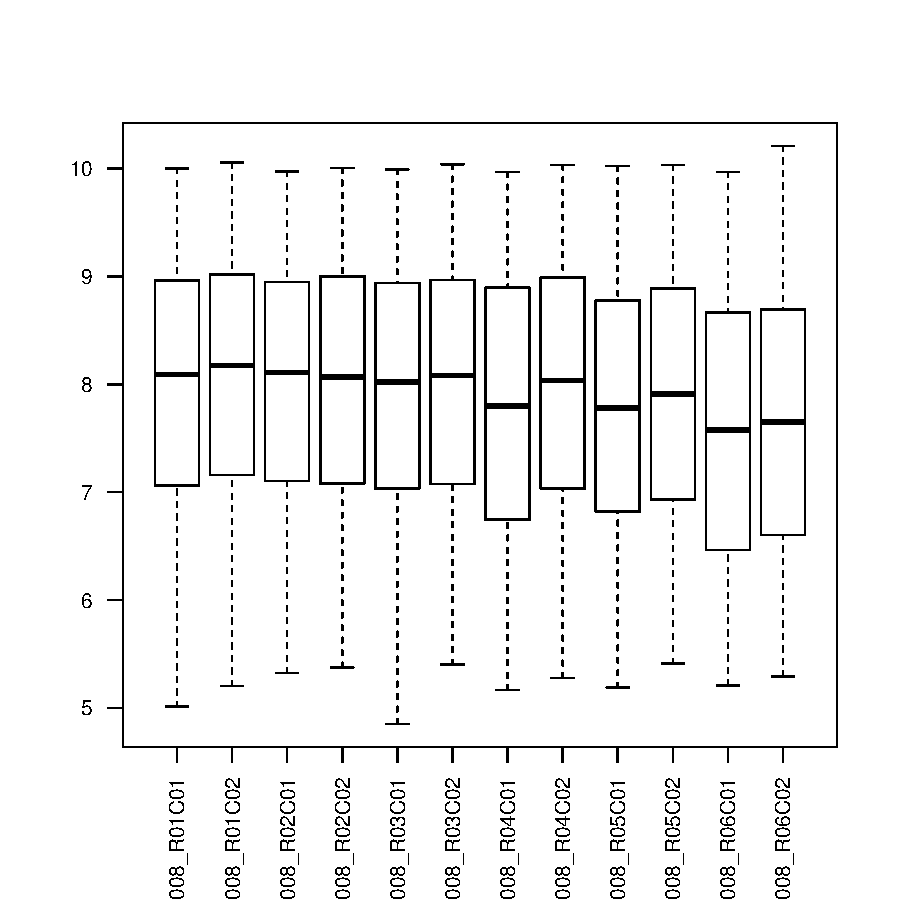
\includegraphics{wateRmelon-IncludeGraphic}
\begin{Schunk}
\begin{Sinput}
> boxplot(log(unmethylated(melon)), las=2, cex.axis=0.8 )
\end{Sinput}
\end{Schunk}
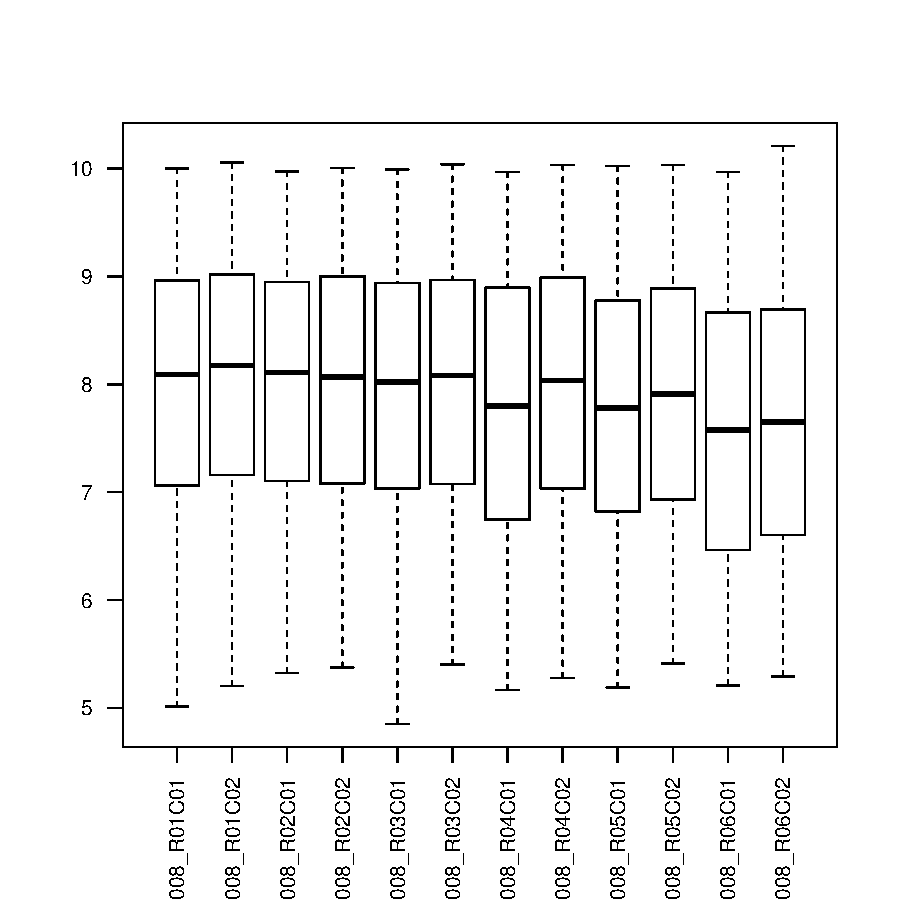
\includegraphics{wateRmelon-IncludeGraphic}

Filtering by detection p-value provides a straightforward 
approach for removing both failed samples and probes.  
The \Rfunction{pfilter} function
conveniently discards samples with more than (by default ) 1\% of 
probes above the .05 detection p-value threshold, and probes with any samples
with beadcount under 3 or more than 1\% above the p-value threshold.

\begin{Schunk}
\begin{Sinput}
> melon.pf <- pfilter(melon)
\end{Sinput}
\begin{Soutput}
0 samples having 1 % of sites with a detection p-value greater than 0.05 were removed 
Samples removed:  
72 sites were removed as beadcount <3 in 5 % of samples 
40 sites having 1 % of samples with a detection p-value greater than 0.05 were removed 
\end{Soutput}
\end{Schunk}

It has come to our attention that data read in using the various packages and 
input methods will give subtly variable data output as they 
calculate detection p-value and beta values differently, and do/don?t give 
information about beadcount.  The pfilter function does not correct 
for this, but simply uses the detection p-value and bead count 
provided by each package.

\subsection{Normalize and calculate betas}

In our analysis[1] we tested 15 preprocessing and normalization methods.  
This involved processing 10 data sets 15 different ways and calculating three
metrics of performance from each one.  You can do the same thing with 
your data if you like, but our recommended method \Rfunction{dasen}
will work well for most data sets.  If you suspect varying dye bias (if
you have arrays scanned on different instruments, for example), you might 
want to try \Rfunction{nanes}.

\begin{Schunk}
\begin{Sinput}
> melon.dasen.pf <- dasen(melon.pf)
\end{Sinput}
\end{Schunk}

\subsection{Example workflow: method for MethyLumiSet}
\begin{Schunk}
\begin{Sinput}
> data(melon)		                     
> # load in melon dataset
> melon.pf<-pfilter(melon)	         
\end{Sinput}
\begin{Soutput}
0 samples having 1 % of sites with a detection p-value greater than 0.05 were removed 
Samples removed:  
72 sites were removed as beadcount <3 in 5 % of samples 
40 sites having 1 % of samples with a detection p-value greater than 0.05 were removed 
\end{Soutput}
\begin{Sinput}
> # perform QC on raw data matrix using default thresholds
> melon.dasen.pf<-dasen(melon.pf)	   
> # preprocess using our best method 
> sex  <- pData(melon.dasen.pf)$sex	
> # extract phenotypic information for test
> bet<-betas(melon.dasen.pf)		    
> # extract processed beta values
> melon.sextest<-sextest(bet,sex)	   
> # run t-test to idenitify sex difference
\end{Sinput}
\end{Schunk}

\subsection{Further analysis}
We can't offer much help with the actual analysis, which will be different 
for every experiment.  In general though, you need to get your experimental
variables into the same order as your arrays and apply some kind of statistical
test to each row of the table of betas.  In the workflow shown here, the
array barcodes are preserved and can be retrieved with \Rfunction{sampleNames} 
or \Rfunction{colnames}.  It's convenient to read in a samplesheet, for
example in csv format, with the barcodes as row names.

\section{References}
[1] Pidsley R, Wong CCY, Volta M, Lunnon K, Mill J, Schalkwyk LC: 
A data-driven approach to preprocessing Illumina 450K methylation 
array data (submitted)

[2] Dedeurwaerder S, Defrance M, Calonne E, Sotiriou C, Fuks F: 
Evaluation of the Infinium Methylation 450K technology . Epigenetics 
2011, 3(6):771-784.

[3] Touleimat N, Tost J: Complete pipeline for Infinium R Human 
Methylation 450K BeadChip data processing using subset quantile 
normalization for accurate DNA methylation estimation. Epigenomics 
2012, 4:325-341)

[4]Teschendorff AE, Marabita F, Lechner M, Bartlett T, Tegner J, Gomez-Cabrero D,
Beck S. A Beta-Mixture Quantile Normalisation method for correcting probe design 
bias in Illumina Infinium 450k DNA methylation data. Bioinformatics. 2012 Nov 21.

[5] Maksimovic J, Gordon L, Oshlack A: SWAN: Subset quantile 
Within-Array Normalization for Illumina Infinium HumanMethylation450 
BeadChips. Genome biology 2012, 13(6):R44


\end{document}

% R CMD Sweave waternette.rnw
% R CMD texi2dvi --pdf --clean waternette.tex
% R CMD Stangle waternette.rnw
